\documentclass{article}
\usepackage[utf8]{inputenc}
\usepackage{natbib}
\usepackage[T1]{fontenc}
\usepackage[francais]{babel}
\usepackage{chemist}
\usepackage{array}
\usepackage[version=3]{mhchem}
\usepackage{amsmath}
\usepackage[squaren,Gray]{SIunits}
\usepackage{numprint}
\usepackage{amsfonts}
\usepackage{amssymb}
\usepackage{graphicx}
\usepackage{mathtools}
\usepackage{fullpage}
\usepackage{mhchem}
\usepackage{listings}
\usepackage{hyperref}
\usepackage{mathenv} %%%%%%%%%%% do not forget to add to head.tex
\usepackage{empheq} %%%%%%%%%%%% same
\author{Groupe 1246 }


\title{\vspace{\fill}\begin{LARGE} \begin{bf}
Rapport de la quatrième tâche: Analyse de sécurité ciblée sur une des unités de production\\
LFSAB1503 \\
\end{bf}\end{LARGE}
\vspace{\fill}}
\begin{document}
\maketitle
\newpage
\tableofcontents
\newpage
\newpage
\section{Introduction}

	Cette quatrième tâche présente une analyse, selon la procédure \textsc{Hazop}, des risques liés au fonctionnement 
du réacteur de synthèse de l’ammoniac. Cette tâche a été principalement rédigée lors de la séance tutorée en S10. Le rapport 
se divise comme suit: Dans un premier lieu, nous rappellerons ce qu'est une procédure \textsc{Hazop}, son utilité ainsi 
que sa structure. Ensuite, nous proposerons une mini-\textsc{Hazop} pour une section de notre procédé: la synthèse même 
de l'ammoniac. Les risques ne seront pas estimés quantitativement.

\section{Analyse \textsc{Hazop}}

\subsection{Section du procédé analysé et composants utilisés}
\begin{table}[ht!]
 \centering
 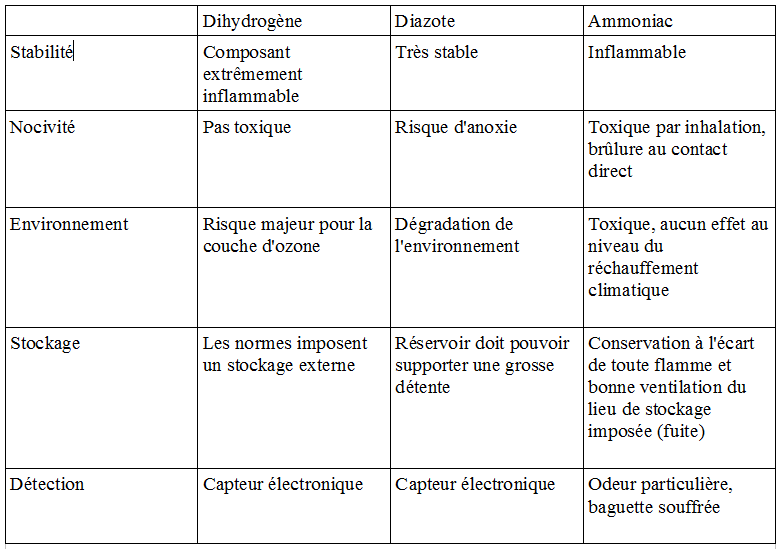
\includegraphics[scale=0.6]{TabComp.PNG}
 \caption{Comparaison des différents composants en réaction}
 \label{TabComp}
\end{table}

Nous n'avons réalisé qu'une \textsc{Hazop} partielle de notre procédé de production d'ammoniac. Nous n'avons considéré 
que la dernière étape du procédé, c'est-à-dire la réaction de synthèse d'ammoniac. La section du procédé peut être visualisée 
sur la Figure \ref{section_procede}. Il apparaît dès lors que les seuls composants étudiés sont le diazote, le dihydrogène 
et l'ammoniac. Afin d'effectuer une analyse de risques, il est nécessaire de réaliser une pré-étude concernant ces composés 
et leurs dangers potentiels. Nous avons résumé tout cela dans le Tableau \ref{TabComp}.\cite{CSST}\cite{Ontario}

\begin{figure}[ht!]
 \centering
 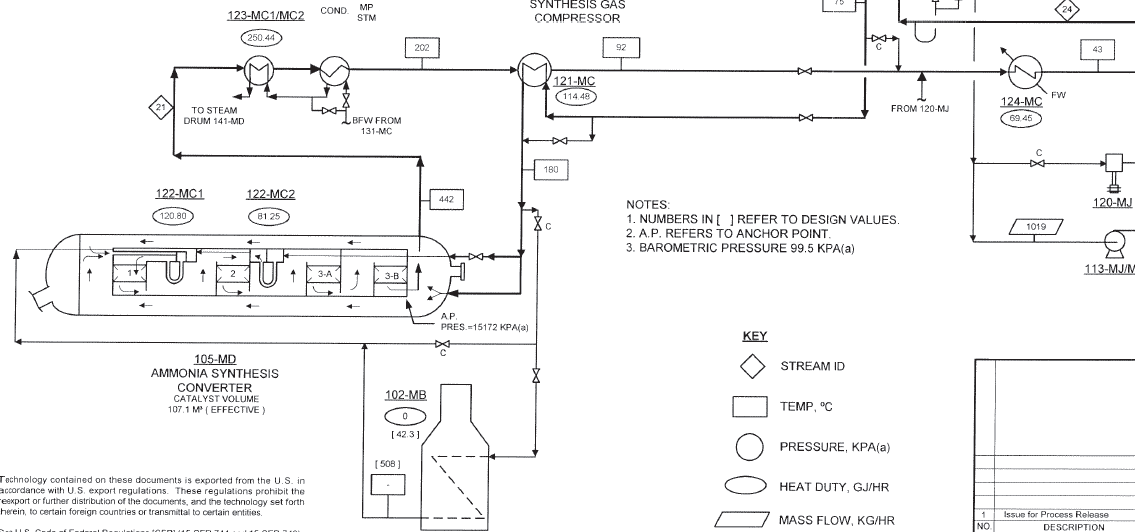
\includegraphics[scale=0.3]{section_procede.PNG}
 \caption{Section du procédé étudiée}
 \label{section_procede}
\end{figure}

\subsection{La procédure \textsc{Hazop}}

L’objectif de l’\textsc{Hazop} est d’identifier et d’évaluer les dangers liés au procédé et de déterminer les problèmes 
d’opérations préjudiciables à la marche de l’unité et à la qualité des produits finis. Une telle analyse est nécessaire 
en entreprise étant donné que certaines substances dangereuses sont parfois utilisées, il peut y avoir des activités 
humaines importantes autour des installations, et tout ce qui concerne la sécurité et l'anticipation est très réglementé.
Une \textsc{Hazop} tourne autour d'une structure de noeuds et de mots-clefs très concis et explicites. Cela rend l'analyse 
plus facilement compréhensible et très efficace.
Une telle analyse doit se réitérer de nombreuses fois durant la démarche de conception d'un projet.\cite{icamp}

\paragraph{Questions de départ} Pour réaliser cette analyse \textsc{Hazop}, nous nous sommes basés sur les quelques questions 
suivantes:
\begin{enumerate}
\item Comment les flux de matière circulent-ils dans la section en question et au sein du réacteur de conversion?
Utilisez des surligneurs pour indiquer ces circulations sur le PFD et sur les PIDs de la section. Seules
les circulations concernant le procédé en régime seront prises en compte.
\item Pourquoi n’y a-t-il pas de soupape de sécurité ou de disque de rupture (les deux types de dispositifs
servent à protéger un équipement ou une ligne contre les surpressions) sur le réacteur de synthèse du \ce{NH_3}?
\item Pourquoi y a-t-il des disques de rupture sur l’échangeur 124-MC?
\end{enumerate}

\paragraph{Elements de réponse} La première question a été traitée en séance. Par conséquent, nous ne nous y attarderons 
plus. Les deux autres questions sont des pistes pour trouver quelques endroits sensibles dans le procédé.

\begin{enumerate}
\item Traité en séance.
\item Nous n'avons pas de risque de surpression. Premièrement, étant donné que la réaction de formation de \ce{NH_3} tend à
réduire le nombre de moles de gaz, elle tend à réduire la pression. Par conséquent, nous n'aurons pas d'augmentation de
pression en activité, il n'est donc pas nécessaire de gérer cette augmentation. Deuxièmement, nous pouvons mentionner le
fait qu'une augmentation de la pression va seulement provoquer une augmentation de la vitesse de déplacement du gaz, étant
donné qu'il circule "librement" sur toute cette partie du circuit.
\item Les disques de rupture fonctionnent de la manière suivante: ils
redirigent le contenu du shell vers un tank sécurisé. L'échangeur 124MC peut être assimilé à un radiateur: 
il est compose d'un shell et d'une série de tubes qui le traversent; le but étant un échange de chaleur entre le 
contenu du shell et les tubes. Le shell est rempli d'eau et peut supporter une pression de plus au moins \unit{15}{bar}. 
Les tubes par contre contiennent le gaz à \unit{150}{bar} environ qui vient du réacteur. Dès lors, si un de ces tuyaux 
venait à se briser, son contenu se répandrait et donc la pression maximale que l'enveloppe peut contenir sera dépassée. 
Ceci provoquerait une explosion de l'enveloppe; chose que les disques de rupture permettent justement d'éviter. 
\end{enumerate}

\paragraph{Analyse \textsc{Hazop}} Le tableau \ref{Hazop} reprend quelques scénarios possibles, analysés de la 
manière \textsc{Hazop}.
\begin{landscape}
\begin{table}
\centering
\begin{tabular}{|p{2cm}|p{3cm}|p{4cm}|p{6cm}|p{5cm}|}
\hline
Noeud & Mot guide & Cause & Conséquence & Mesures \\
\hline
\hline
Entrée A2 Réacteur 105MD & LESS/NO FLOW & Vanne HV1046 pas assez ouverte & Mauvais refroidissement au sein du
réacteur & Alarme \\
& & & & \\
& & & Augmentation de la température dans le réacteur & Dispositif d'ouverture automatique \\
& & & & \\
& & & Augmentation dans la sortie B du réacteur & \\
& & & & \\
& MORE FLOW & Vanne HV1046 trop ouverte & Plus de refroidissement au niveau des lits & Alarme \\
& & & Diminution de la température au sein du réacteur & Dispositif de fermeture automatique \\
& & & & \\
& & & Pas de conséquence en terme de sécurité & \\
& & & & \\
& REVERSE FLOW & Pas considéré & Pas considéré & Pas considéré \\
& & & & \\
& & & & \\
& & & & \\
Shell échangeur calorifique 124MC & MORE PRESSURE & Rupture du tube interne (le gaz se répend dans l'enceinte de
l'échangeur & Contamination & Alarme \\
& & & & \\
& & & Risque d'explosion de l'échangeur & Activation du disque de rupture + Déversement dans réservoir alternatif sûr \\
& & & & \\
& LESS PRESSURE & Fuite dans le shell & Perte d'eau & Alarme \\
& & & & \\
& & & Mauvais refroidissement & Réparation \\
& & & & \\
\hline
\end{tabular}
\caption{HAZOP}
\label{Hazop}
\end{table}
\end{landscape}

\newpage
\section{Conclusion}
Au terme de cette analyse, nous pouvons remettre l'accent sur l'importance d'une telle démarche: analyser les risques est 
indispensable durant toute création de projet. Il y a énormément de paramètres à prendre en compte, énormément de tests à 
effectuer, et une infinité de cas à envisager. Les risques n'ont pas été estimés ici quantitativement, 
mais rien qu'une approche qualitative nous permet déjà de visualiser l'ampleur du travail que représente une 
analyse \textsc{Hazop}, ainsi que tous les danger présents dans notre procédé de production d'ammoniac.

\nocite{*}
\bibliographystyle{plain} % Le style est mis entre accolades.
\bibliography{sources} % mon fichier de base de données s'appelle bibli.bib
\end{document}
